\documentclass[10pt, compress]{beamer}

\usepackage{booktabs}
\usepackage[scale=2]{ccicons}
\usepackage{url}
\usepackage{ drawstack }

\graphicspath{ {./pix/} }
\usetheme[useTitleProgressBar]{m}

\title{Radare2}
\subtitle{First r2babies steps - Long Version}
\author{Maxime Morin (@Maijin212), Anton Kochkov (@akochkov)}
\date{\today}
\institute{BSides Las Vegas}

\begin{document}
\maketitle

\begin{frame}[fragile]
  \frametitle{About me}
    \begin{itemize}
    \item 22 y/o french expat @ Luxembourg
    \item Food, Travel and Languages <3
    \item I hate Bullshit
    \item Malware.lu CERT team leader (2days/week) and incident response @ European Commission CSIRC (3days/week)
    \item User of radare2 (impossibru!)
    \item I'm creating tests + documentation
    \end{itemize}
\end{frame}

\begin{frame}[fragile]
  \frametitle{Generality on radare2 framework}
  \begin{itemize}
  \item r1 2006, r2 2009
  \item Multi-(OSes|Archs|Bindings|FileFormats|...)
  \item 10 tools based on the framework
  \item Around 111 contributors from various fields
  \item GSOC + RSOC
  \item CLI/VisualMode/GUI/WebGUI
  \item around 350K LOC
  \end{itemize}
\end{frame}

\plain{Installation !}

\begin{frame}[fragile]
  \frametitle{Installation}
  \begin{itemize}
  \item Always use git version!
  \item Use the provided VM on SSH (\alert{radare:radare} / \alert{root:radare})
  \item git clone \alert{http://github.com/radare/radare2 \&\& cd radare2 \&\& ./sys/install.sh}
  \item Use the Windows installer \alert{http://bin.rada.re/radare2.exe}
  \end{itemize}
\end{frame}

\section{Utilities}

\begin{frame}[fragile]
  \frametitle{Utilities}
     \begin{itemize}
        \item rax2
        \item rabin2
        \item rasm2
        \item radiff2
        \item rafind2
        \item rahash2
        \item radare2
        \item rarun2
        \item ragg2/ragg2-cc
      \end{itemize}
\end{frame}

\begin{frame}[fragile]
  \frametitle{Utilities}
     \begin{itemize}
        \item \alert{rax2}
        \item rabin2
        \item rasm2
        \item radiff2
        \item rafind2
        \item rahash2
        \item radare2
        \item rarun2
        \item ragg2/ragg2-cc
      \end{itemize}
\end{frame}

\begin{frame}[fragile]
  \center\textbf{rax2} — Base converter
  \noindent\makebox[\linewidth]{\rule{\paperwidth}{0.4pt}}
  \frametitle{Utilities: rax2}
  \begin{verbatim}$ rax2 10\end{verbatim}
  \alert{0xa}
  \begin{verbatim}$ rax2 33 0x41 0101b\end{verbatim}
  \alert{0x21 65 0x5}
  \begin{verbatim}$ rax2 -s 4142434445\end{verbatim}
  \alert{ABCDE}
  \begin{verbatim}$ rax2 0x5*101b+5\end{verbatim}
  \alert{30}

\end{frame}

\begin{frame}[fragile]
  \frametitle{Utilities}
     \begin{itemize}
        \item rax2
        \item \alert{rabin2}
        \item rasm2
        \item radiff2
        \item rafind2
        \item rahash2
        \item radare2
        \item rarun2
        \item ragg2/ragg2-cc
      \end{itemize}
\end{frame}

\begin{frame}[fragile]
  \center\textbf{rabin2} — Binary program info extractor
  \noindent\makebox[\linewidth]{\rule{\paperwidth}{0.4pt}}
  \frametitle{Utilities: rabin2}
  \begin{verbatim}$ rabin2 -e\end{verbatim}
  \alert{Entrypoints}
  \begin{verbatim}$ rabin2 -i\end{verbatim}
  \alert{Shows imports}
  \begin{verbatim}$ rabin2 -zz\end{verbatim}
  \alert{Shows strings}
  \begin{verbatim}$ rabin2 -g\end{verbatim}
  \alert{Show all possible information}

\end{frame}

\begin{frame}[fragile]
  \frametitle{Utilities}
     \begin{itemize}
        \item rax2
        \item rabin2
        \item \alert{rasm2}
        \item radiff2
        \item rafind2
        \item rahash2
        \item radare2
        \item rarun2
        \item ragg2/ragg2-cc
      \end{itemize}
\end{frame}

\begin{frame}[fragile]
  \center\textbf{rasm2} — assembler and disassembler tool
  \noindent\makebox[\linewidth]{\rule{\paperwidth}{0.4pt}}
  \frametitle{Utilities: rasm2}
  \begin{verbatim}$ rasm2 -a x86 -b 32 'mov eax, 33'\end{verbatim}
  \alert{Assemble}
  \begin{verbatim}$ rasm2 -d 9090\end{verbatim}
  \alert{Disassemble}
  \begin{verbatim}$ rasm2 -L\end{verbatim}
  \alert{List supported asm plugins}
  \begin{verbatim}$ rasm2 -a x86 -b 32 'mov eax, 33' -C\end{verbatim}
  \alert{Output in C format}

\end{frame}

\begin{frame}[fragile]
  \frametitle{Utilities}
     \begin{itemize}
        \item rax2
        \item rabin2
        \item rasm2
        \item \alert{radiff2}
        \item rafind2
        \item rahash2
        \item radare2
        \item rarun2
        \item ragg2/ragg2-cc
      \end{itemize}
\end{frame}

\begin{frame}[fragile]
  \center\textbf{radiff2} — unified binary diffing utility
  \noindent\makebox[\linewidth]{\rule{\paperwidth}{0.4pt}}
  \frametitle{Utilities: radiff2}
  \begin{verbatim}$ radiff2 original patched\end{verbatim}
  \alert{Code diffing}
  \begin{verbatim}$ radiff2 -C original patched\end{verbatim}
  \alert{Code diffing using graphdiff algorithm}
  \begin{verbatim}$ radiff2 -g main -a x86 -b32 original patched\end{verbatim}
  \alert{Graph diff output of given symbol, or between two functions, at given offsets: one for each binary.}

\end{frame}

\begin{frame}[fragile]
\frametitle{Utilities: radiff2 — graph example}
  \begin{figure}
\begin{center}/bin/true\hfill /bin/false\end{center}
  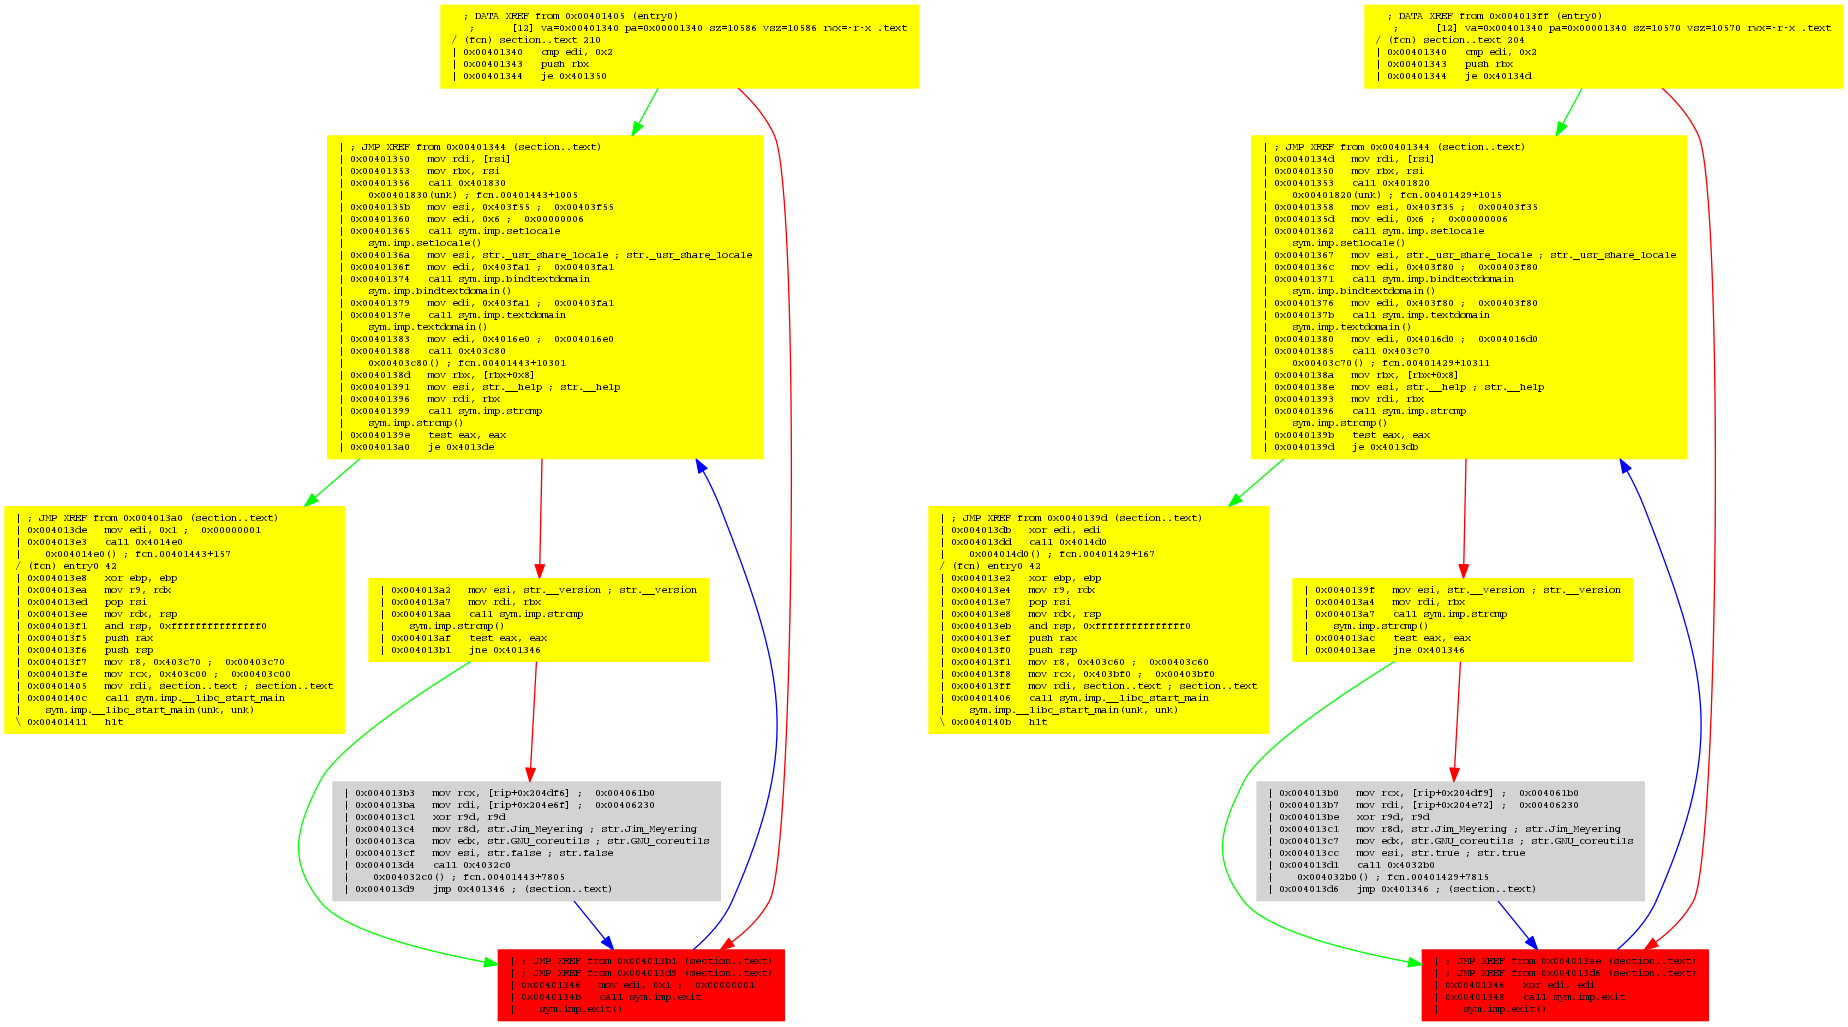
\includegraphics[width=\textwidth]{radiff2.png}
  \end{figure}
\end{frame}

\begin{frame}[fragile]
  \frametitle{Utilities}
     \begin{itemize}
        \item rax2
        \item rabin2
        \item rasm2
        \item radiff2
        \item \alert{rafind2}
        \item rahash2
        \item radare2
        \item rarun2
        \item ragg2/ragg2-cc
      \end{itemize}
\end{frame}

\begin{frame}[fragile]
  \center\textbf{rafind2} — Advanced commandline hexadecimal editor
  \noindent\makebox[\linewidth]{\rule{\paperwidth}{0.4pt}}
  \frametitle{Utilities: rafind2}
  \begin{verbatim}$ rafind2 -X -s passwd dump.bin\end{verbatim}
  \alert{Search for the string passwd}

\end{frame}

\begin{frame}[fragile]
  \frametitle{Utilities}
     \begin{itemize}
        \item rax2
        \item rabin2
        \item rasm2
        \item radiff2
        \item rafind2
        \item \alert{rahash2}
        \item radare2
        \item rarun2
        \item ragg2/ragg2-cc
      \end{itemize}
\end{frame}

\begin{frame}[fragile]
  \center\textbf{rahash2} — block based hashing utility
  \noindent\makebox[\linewidth]{\rule{\paperwidth}{0.4pt}}
  \frametitle{Utilities: rahash2}
  \begin{verbatim}$ rahash2 -a all binary.exe\end{verbatim}
  \alert{Display hashes of the whole file with all algos}
  \begin{verbatim}$ rahash2 -B -b 512 -a md5\end{verbatim}
  \alert{Compute md5 per block of 512}
  \begin{verbatim}$ rahash2 -B -b 512 -a entropy\end{verbatim}
  \alert{Compute md5 per block of 512}
  \begin{verbatim}$ echo -n "admin" | rahash2 -a md5 -s "\end{verbatim}
  \alert{Compute md5 of the string admin}

\end{frame}

\begin{frame}[fragile]
  \frametitle{Utilities}
     \begin{itemize}
        \item rax2
        \item rabin2
        \item rasm2
        \item radiff2
        \item rafind2
        \item rahash2
        \item \alert{radare2}
        \item rarun2
        \item ragg2/ragg2-cc
      \end{itemize}
\end{frame}

\section{Radare2 — Command line}

\begin{frame}[fragile]
  \frametitle{1 command <—> 1 Reverse-Engineering'notion}
  Keep in mind that:
  \begin{enumerate}
  \item Every character has a meaning i.e \alert{(w = write, p = print)}
  \item Every command is a succession of character i.e \alert{pdf = p <-> print d <-> disassemble f <-> function }
  \item Every command is documented with \textbf{cmd?}, i.e \alert{pdf?},\alert{?}, \alert{???}, \alert{???}, \alert{?\$?}, \alert{?@?}
  \end{enumerate}
\end{frame}

\begin{frame}[fragile]
  \frametitle{The \# command — hashing command}
  \begin{enumerate}
  \item Open a file with radare2 \alert{radare2 file.exe}
  \item Get Usage on the command \alert{\#?} \textbf{Usage: \#algo <size> @ addr}
  \item List of all existing algorithms \alert{\#\#}
  \item SHA1 \alert{\#sha1}
  \item Hashing from the begin \alert{\#sha1 @ 0}
  \item with a hash block size corresponding to the size of the file \alert{\#sha1 \$s @ 0x0}
 \end{enumerate}
This command is same as rahash2 -a sha1 file.exe
\end{frame}

\begin{frame}[fragile]
  \frametitle{The i command — information command}
  \begin{enumerate}
  \item Get Usage on the command \alert{i?}
  \item Same as \alert{rabin2}
  \item izj for displaying in json
  \item internal commands: \~, ls, \{\}, ..
 \end{enumerate}
\end{frame}

\begin{frame}[fragile]
  \frametitle{Radare2 — 'Major' command example: pf}
  Quick Demo
\end{frame}

\begin{frame}[fragile]
  \frametitle{The t command — types management}
  \begin{enumerate}
  \item Get Usage on the command \alert{t?}
  \item 'to' to load the types from the C header file
  \item tl link type to the memory, tf shows it like the pf
  \item add 'j' to get the output in the json format
 \end{enumerate}
\end{frame}

% This demo is in demos/demo3_x86_legacy
% 1. Open 'r2 -a x86 asrock_p4i65g.bin'  - it should recognize legacy BIOS format automatically
% (x86, 16bit)
% 2.'[f000:fff0]> . asrock_p4i65g.r2' - add some comments and functions in the loaded fresh file
% 3.'[f000:4736]> to asrock_p4i65g.h'
% 4.'[f000:4736]> t' - list all loaded types
% 5.'[f000:4736]> s SIO_Init' - go to the SIO_Init() function address
% 6.'[f000:5c93]> Vp' - show the code, tell that lines mov si, 0x5c50 ; lodsw ax, word cs:[si] is
% actually reading some data, after some background research we've found this is a table of the
% SuperIO registers, so we can apply structure here, to see the values
% 7.'[f000:5c93]> tl SIO_reg_mask 0xf000:0x5c50' - link the structure 'SIO_reg_mask' to the 0xf000:0xfc50 address
% 8.'[f000:5c93]> tf 0xf000:0x5c50' - shows the values (be careful, there is a bug, don't attract
% attention that it shows dwords instead of chars (should be char) from the structure description.

% Additional information here http://radare.today/types/

\begin{frame}[fragile]
  \frametitle{Radare2 - types command example}
  Quick Demo
\end{frame}

\begin{frame}[fragile]
  \frametitle{Radare2 — CLI Main commands}
  \begin{enumerate}
   \item r2 -A or r2 then aaa : Analysis
   \item s : Seek
   \item pdf : Print disassemble function
   \item af? : Analyse function
   \item ax? : Analyse XREF
   \item /? : Search
   \item ps? : Print strings
   \item C? : Comments
   \item w? : Write
 \end{enumerate}
\end{frame}

\section{Radare2 — Visual mode}
\begin{frame}[fragile]
  \frametitle{Radare2 — Visual mode Main commands}
  \begin{enumerate}
  \item V? : Visual help
  \item p/P : rotate print modes
  \item move using arrows/hjkl
  \item o : seek to
  \item e : r2configurator
  \item v : Function list
  \item \_ : HUD
  \item V : ASCII Graph
 \end{enumerate}
\end{frame}

\section{Radare2 — WebUI}
\begin{frame}[fragile]
  \frametitle{Radare2 — WebUI}
  r2 -A -c=H filename
    \begin{figure}
  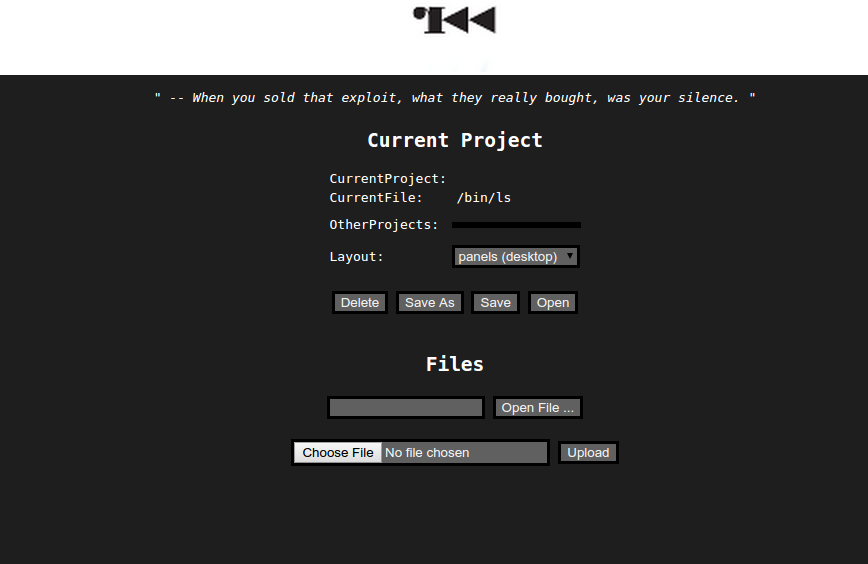
\includegraphics[width=\textwidth]{web.png}
  \end{figure}
\end{frame}

\section{Radare2 — Debugger}

\begin{frame}[fragile]
  \frametitle{Radare2 — Debugger}
  \begin{enumerate}
  \item radare2 -d
  \item Quickly switch to Visual debugger mode: Vpp
  \item OllyDBG/IDApro shortcuts friendly
 \end{enumerate}
\end{frame}

\begin{frame}[fragile]
  \frametitle{Utilities}
     \begin{itemize}
        \item rax2
        \item rabin2
        \item rasm2
        \item radiff2
        \item rafind2
        \item rahash2
        \item radare2
        \item \alert{rarun2}
        \item ragg2/ragg2-cc
      \end{itemize}
\end{frame}

\begin{frame}[fragile]
  \frametitle{Rarun2}
  \center\textbf{Rarun2} — run programs in exotic environments
  \noindent\makebox[\linewidth]{\rule{\paperwidth}{0.4pt}}
  \begin{enumerate}
  \item Environnment setup tools for radare2
  \item most useful with debugger
  \item aslr, stdout, arguments, r2preload ...
 \end{enumerate}
\end{frame}

\begin{frame}[fragile]
  \frametitle{Utilities}
     \begin{itemize}
        \item rax2
        \item rabin2
        \item rasm2
        \item radiff2
        \item rafind2
        \item rahash2
        \item radare2
        \item rarun2
        \item \alert{ragg2/ragg2-cc}
      \end{itemize}
\end{frame}

\begin{frame}[fragile]
  \frametitle{Ragg2/Ragg2-cc}
  \center\textbf{Ragg2/Ragg2-cc} — frontend for compiling shellcodes
  \noindent\makebox[\linewidth]{\rule{\paperwidth}{0.4pt}}
\end{frame}

\begin{frame}[fragile]
  \frametitle{Debugging}
  \begin{itemize}
	\item Native local debug (r2 -d)
	\item r2 agent (rap:// protocol)
	\item GDB remote protocol support
	\item WinDBG remote protocol support
  \end{itemize}
\end{frame}

\begin{frame}[fragile]
  \frametitle{Native debug}
  \center Better to use the visual mode
  \center r2 -d /bin/ls
  \begin{figure}
  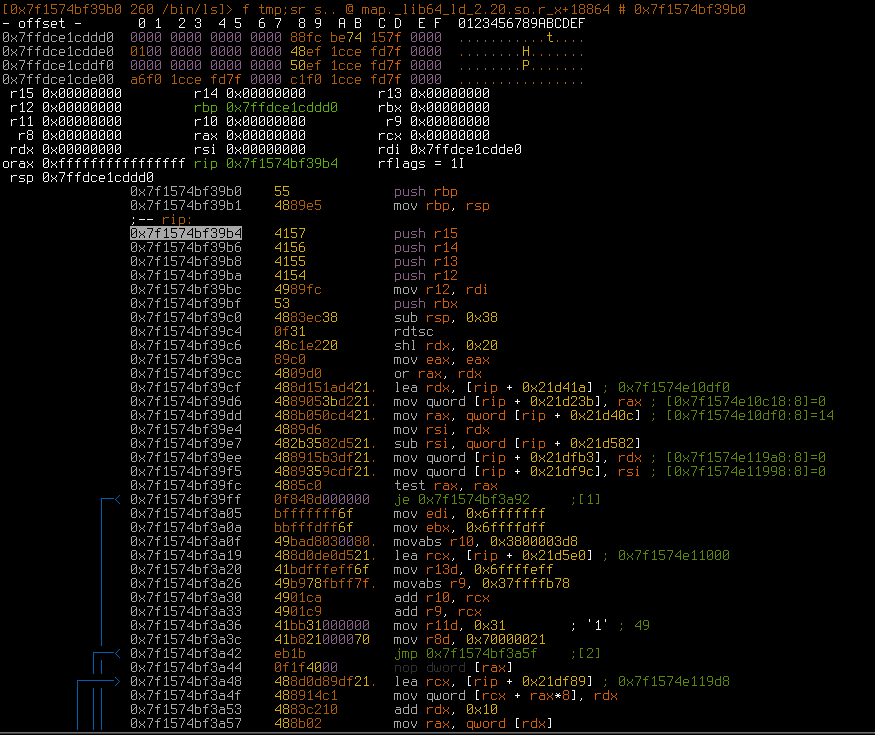
\includegraphics[width=\textwidth]{r2-nativedebug.png}
  \end{figure}
\end{frame}

\begin{frame}[fragile]
  \frametitle{GDB protocol}
  \center Just run gdbserver somewhere
  \center and connect r2 to it:
  \center r2 -D gdb -d /bin/ls gdb://99.44.23.50:4589
\end{frame}

\begin{frame}[fragile]
  \frametitle{GDB protocol + Wine}
  \center Winedbg allows to run windows command
  \center using the gdbserver too:
  \center winedbg --gdb --no-start malware.exe
  \center r2 -a x86 -b 32 -D gdb -d malware.exe gdb://localhost:44840
\end{frame}

\begin{frame}[fragile]
  \frametitle{WinDBG}
  \center r2 allows to connect WinDBG/KD
  \center For example, to debug windows kernel via the serial port:
  \center bcdedit /debug on
  \center bcdedit /dbgsettings serial debugport:1 baudrate:115200
  \center then connect r2:
  \center r2 -a x86 -b 32 -D wind windbg:///tmp/windbg.pipe
  \center For now, connecting to the QEMU and VirtualBox are tested
% More information here https://github.com/radare/radare2/blob/master/doc/windbg
\end{frame}

\begin{frame}[fragile]
  \frametitle{Debugging OMAP BootRom}
  \center Just run it in the modified qemu https://github.com/XVilka/qemu
  \center ./configure --target-list=arm-softmmu ; make ; sudo make install
  \center qemu-system-arm -M milestone -m 256 -L . -bios bootrom.bin -mtdblock	mbmloader-1.raw -d in\_asm,cpu,exec -nographic -s -S
  \center r2 -D gdb -b arm gdb://localhost:9999
  \center Same approach could be used for any customized hardware
\end{frame}

% show demo here - demos/demo1_arm_boot

\begin{frame}[fragile]
  \frametitle{GDB protocol + Wine}
  \center Winedbg allows to run windows command
  \center using the gdbserver too:
  \center winedbg --gdb --no-start malware.exe
  \center r2 -a x86 -b 32 -D gdb -d malware.exe gdb://localhost:44840
\end{frame}

\section{Firmware analysis}
\begin{frame}[fragile]
  \frametitle{UEFI analysis}
  \begin{itemize}
    \item Dump the image using flashrom or hardware
	\item Unpack the image using UEFITool
	\item Open the selected PE or TE file using r2
  \end{itemize}
\end{frame}

% show demo here - demos/demo3_x86_uefi
% download UEFITool here https://github.com/LongSoft/UEFITool

\begin{frame}[fragile]
  \frametitle{Old legacy BIOS analysis}
  % This shows the example of talking to the SMBus
  \begin{itemize}
    \item Load the whole image or unpack it using bios\_extract
	\item Open it using the correct segment and offset
	\item r2 load the whole BIOS image automatically
	\item r2 asrock\_p4i65g.bin
	\item >. asrock\_p4i65g.r2
  \end{itemize}
\end{frame}

% show demo here - demos/demo3_x86_legacy
% download bios_extract here http://www.coreboot.org/Bios_extract

\begin{frame}[fragile]
  \frametitle{Embedded controller - 8051}
  \center Lets start from the static analysis
  \center r2 -a 8051 ite\_it8502.rom
  \center >. ite\_it8502.r2
\end{frame}

% show demo here - demos/demo5_it8502e

\begin{frame}[fragile]
  \frametitle{Embedded controller - 8051 - ESIL VM}
  \center Lets start from the static analysis
  \center r2 -a 8051 ite\_it8502.rom
  \center . ite\_it8502.r2
  \center run 'aei' command to init ESIL VM
  \center run 'aeim' command to init ESIL VM stack
  \center run 'aeip' command to start from the current offset
  \center run 'aecu [addr]' to emulate until the [addr] is reached
\end{frame}
% show demo here
% Reference to the example from here? http://radare.tv/a/44

\begin{frame}[fragile]
  \frametitle{Embedded controller - 8051 - ESIL2REIL}
  \center Lets start again from the same place
  \center r2 -a 8051 ite\_it8502.rom
  \center . ite\_it8502.r2
  \center run 'pae' to show the esil expression
  \center run 'aetr' to convert the esil output to REIL
  \center store this to some file and use the 'openreil' utility to SMT it
\end{frame}
% reference to the https://github.com/Cr4sh/openreil
% what about some demo for that?

\begin{frame}[fragile]
  \frametitle{Scripting Capabilities}
  \center Available for a lot of programming languages
  \center\textbf{Radare2 Bindings} —
  \center\textbf{R2Pipe} —
  \noindent\makebox[\linewidth]{\rule{\paperwidth}{0.4pt}}
  \item Demo time !
\end{frame}

\begin{frame}[fragile]
  \frametitle{Now your turn!}
    \begin{itemize}
    \item \alert{Crackmes:} IOLI-Crackme, flare-on 2015 challenges
    \item \alert{Exploitation:} pwn1, pwn2, ropasaurus
    \item \alert{Malware(1/3):} Practical malware analysis samples
    \item \alert{Malware(2/3):} Any RAT samples see decoder on: https://github.com/kevthehermit/RATDecoders/
    \item \alert{Malware(3/3):} AVCaesar.lu, MalekalDB
    \item \alert{Firmware/BIOS/UEFI:} TODO
    \end{itemize}
\end{frame}

\begin{frame}[fragile]
  \frametitle{Documentation}
    \begin{itemize}
    \item \alert{Website:} http://rada.re/
    \item \alert{Blog:} http://radare.today
    \item \alert{Book:} http://maijin.gitbooks.io/radare2book/content/
    \end{itemize}
\end{frame}

\section{Exploitation (jvoisin work :-) )}

\begin{frame}[fragile]
	\begin{center}
		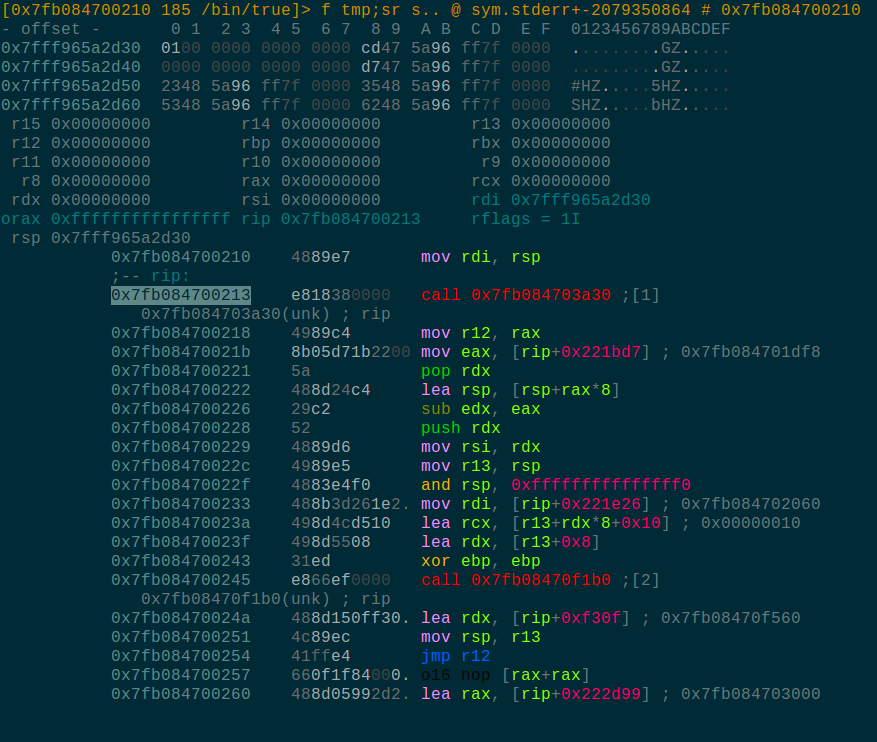
\includegraphics[width=\textwidth]{regstacklisting.png}
	\end{center}
\end{frame}

\begin{frame}{Stack}
	\begin{center}
	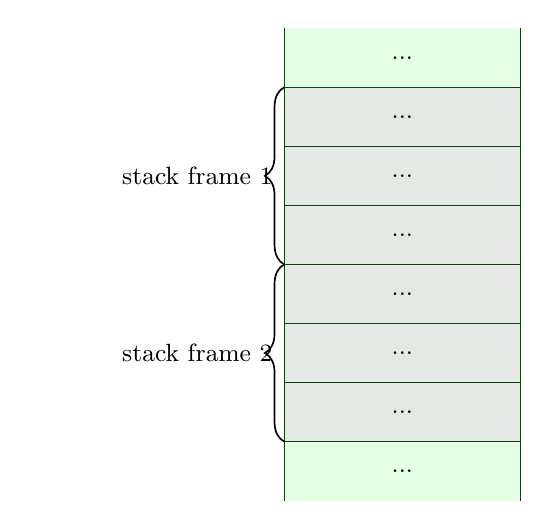
\begin{tikzpicture}[scale=0.75]
		\small
		\stacktop{}
		\startframe
		\padding{1}{...}
		\padding{1}{...}
		\padding{1}{...}
		\finishframe{stack frame 1}
		\startframe
		\padding{1}{...}
		\padding{1}{...}
		\padding{1}{...}
		\finishframe{stack frame 2}
		\stackbottom{}
	\end{tikzpicture}
	\end{center}
\end{frame}

\begin{frame}{Stack smashing}
	\begin{center}
		\begin{columns}
			\begin{column}{.5\textwidth}
				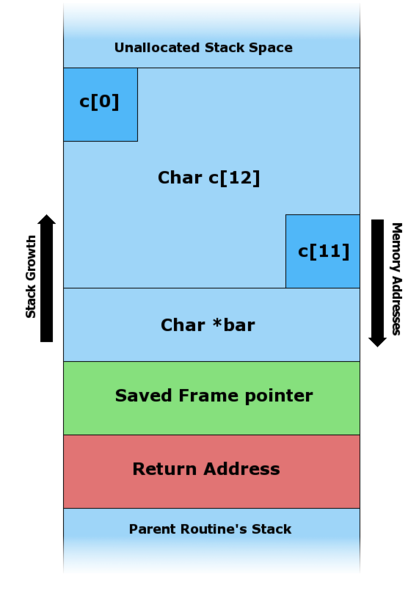
\includegraphics[height=6.5cm]{overflow1.png}
			\end{column}
			\begin{column}{.5\textwidth}
				\only<1>{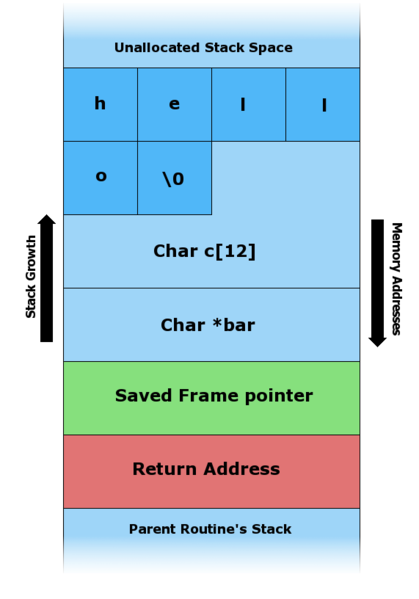
\includegraphics[height=6.5cm]{overflow2.png}}
				\only<2>{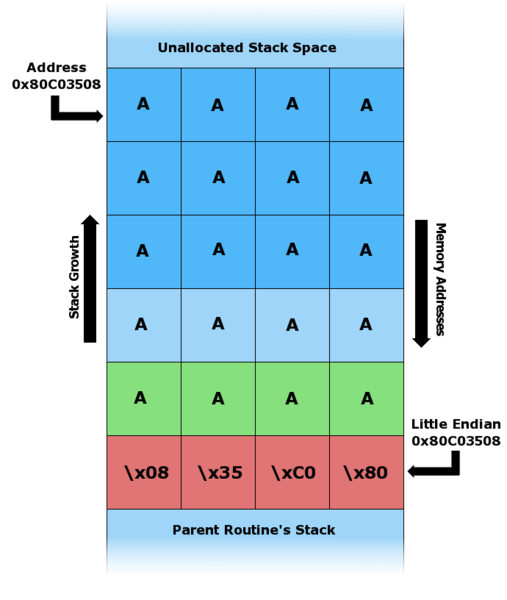
\includegraphics[height=6.5cm]{overflow3.png}}
			\end{column}
		\end{columns}
	\end{center}
\end{frame}

\section{Pwn1}
\begin{frame}{Pwn1}
	\begin{itemize}
		\item Written for this workshop
		\item Oldschool \emph{classic} example
		\item You'll write the final exploit
	\end{itemize}
\end{frame}

\begin{frame}{Hu-ho.}
	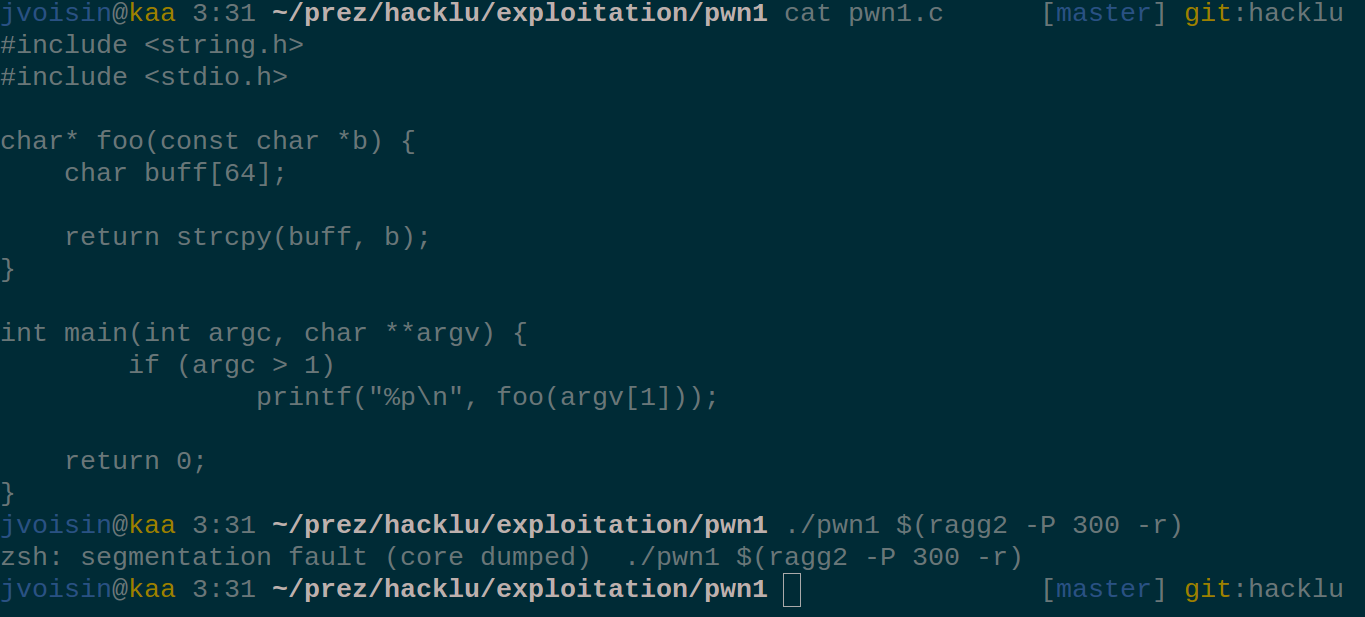
\includegraphics[width=\textwidth,height=6.5cm]{segfault_pwn1.png}
\end{frame}

% Explain what a De Bruijn pattern is
\begin{frame}{De Bruijn patterns}
	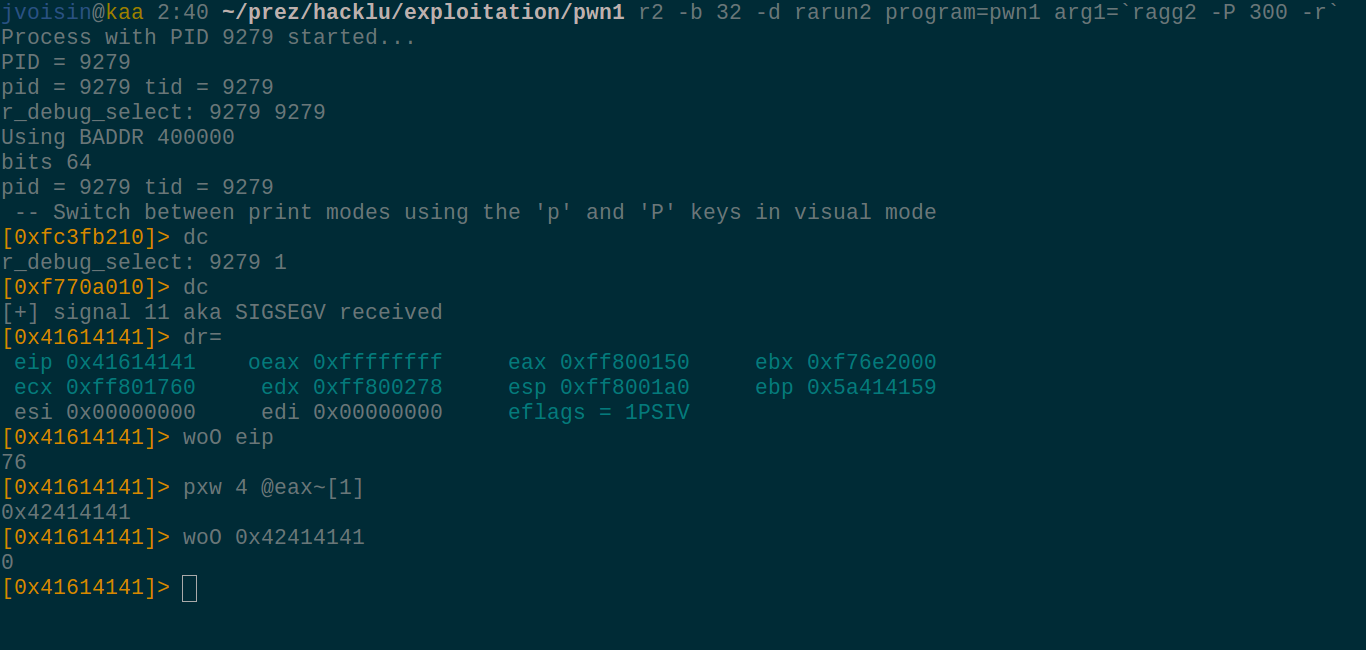
\includegraphics[width=\textwidth,height=6.5cm]{bruijn.png}
\end{frame}

\begin{frame}{Exploit!}
	\begin{columns}
		\begin{column}{.3\textwidth}
			\begin{itemize}
				\item No ALSR
				\item No NX
				\item No Canary
			\end{itemize}
		\end{column}
		\begin{column}{.7\textwidth}
			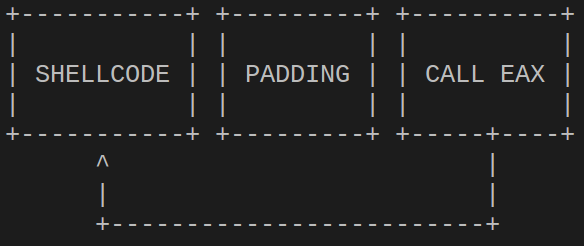
\includegraphics[width=\textwidth,height=2cm]{pwn1_shellcode.png}
		\end{column}
	\end{columns}
\end{frame}

\begin{frame}{Generate shellcode}
	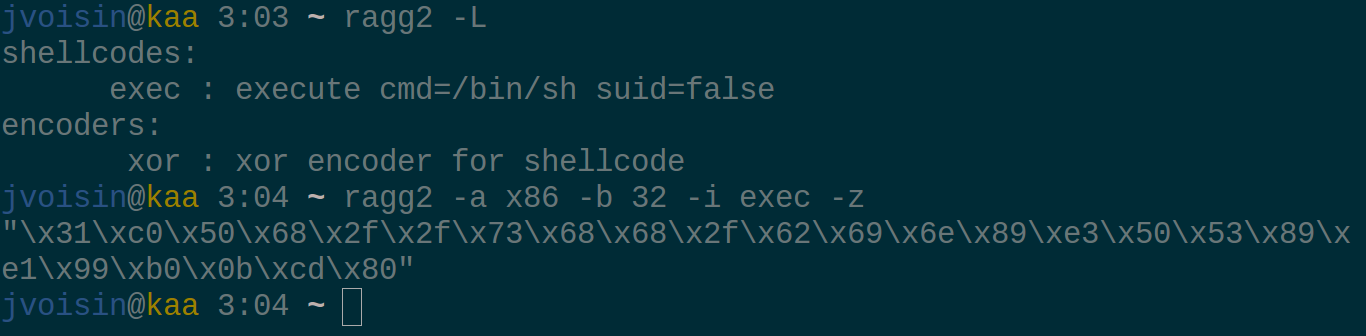
\includegraphics[width=\textwidth]{binsh.png}
	\vskip.5cm
	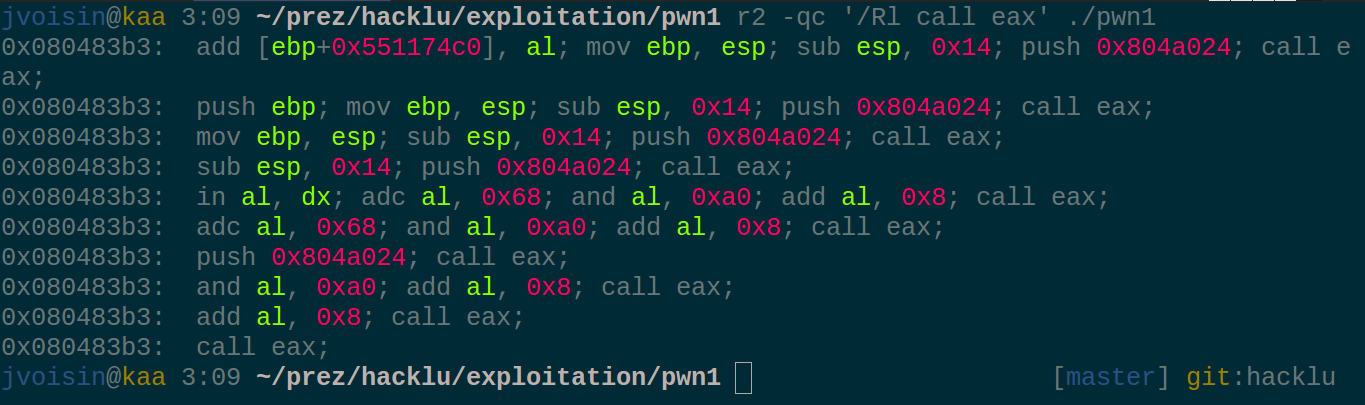
\includegraphics[width=\textwidth]{rop_pwn1.png}
\end{frame}

\begin{frame}{Your turn!}
	\begin{center}
		Write a working exploit!
	\end{center}
\end{frame}

\begin{frame}{Show me yours, I'll show you mine}
	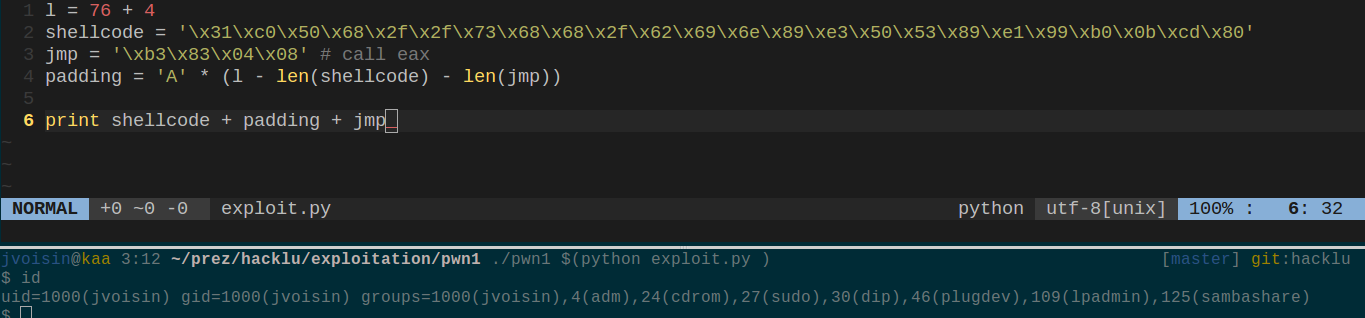
\includegraphics[width=1.05\textwidth,height=4.5cm]{exploit_pwn1.png}
\end{frame}

\section{Malware Analysis}

\begin{frame}[fragile]
  \frametitle{Other r2 commands I use frequently at work}
  \begin{enumerate}
   \item \#?
   \item ?d, i?
   \item Visual mode and associated (VVV, Vv, ;, ...)
   \item Analysis command (axt, agf, ...)
   \item /m?, /C?, pf, px?, p6d, p=
   \item yara, zF
   \item pr, wt
   \item basic zsh/bash scripting, r2-pipe
 \end{enumerate}
\end{frame}

\begin{frame}[fragile]
  \frametitle{Documentation}
    \begin{itemize}
    \item \alert{Website:} http://rada.re/
    \item \alert{Blog:} http://radare.today
    \item \alert{Book:} http://maijin.gitbooks.io/radare2book/content/
    \end{itemize}
\end{frame}

\end{document}
